\renewcommand{\captiontitle}{健康受试者的分割结果}
\begin{figure*}
\begin{center}

\setlength{\tabcolsep}{1pt}

\begin{tabular}{ccccc}

\toprule
\SA{}(底层切片) & \SA{} (中间切片) & \SA{}(顶层切片) & \HLA{} & \VLA{} \\
\midrule

\multicolumn{5}{c}{未对齐方向的原始图像:$\image$} \\

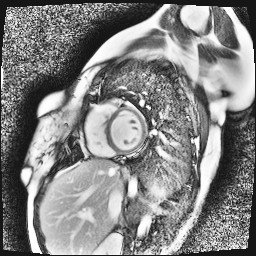
\includegraphics[width=0.19\textwidth]{./data/representative-results/control/HCMNet_2600035/00_SAX/BASE/0.png} &
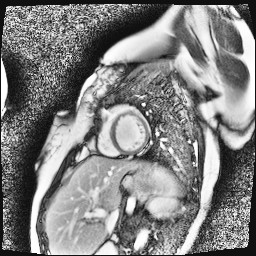
\includegraphics[width=0.19\textwidth]{./data/representative-results/control/HCMNet_2600035/00_SAX/MID/0.png} &
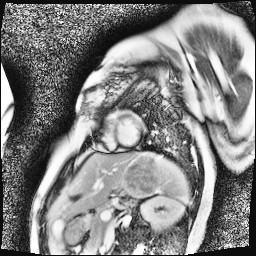
\includegraphics[width=0.19\textwidth]{./data/representative-results/control/HCMNet_2600035/00_SAX/APEX/0.png} &
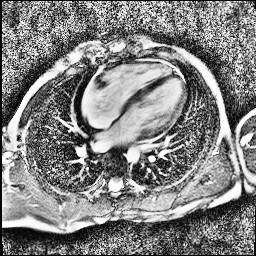
\includegraphics[width=0.19\textwidth]{./data/representative-results/control/HCMNet_1700012/01_HLA/00/0.png} &
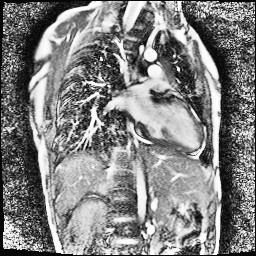
\includegraphics[width=0.19\textwidth]{./data/representative-results/control/HCMNet_1700012/02_VLA/00/0.png} \\

\multicolumn{5}{c}{结构定位} \\

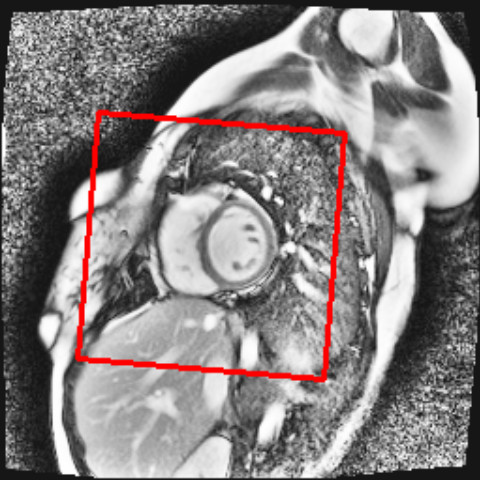
\includegraphics[width=0.19\textwidth]{./data/representative-results/control/HCMNet_2600035/00_SAX/BASE/0_bbox.png} &
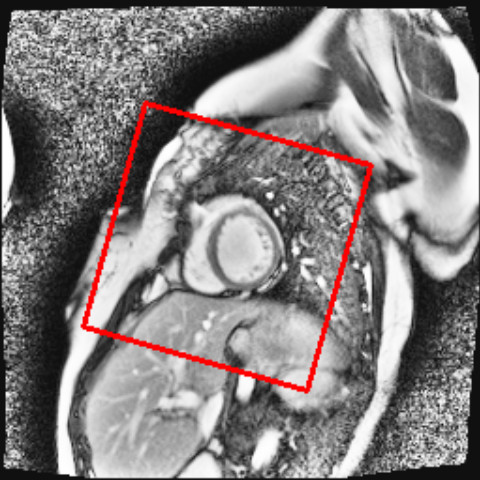
\includegraphics[width=0.19\textwidth]{./data/representative-results/control/HCMNet_2600035/00_SAX/MID/0_bbox.png} &
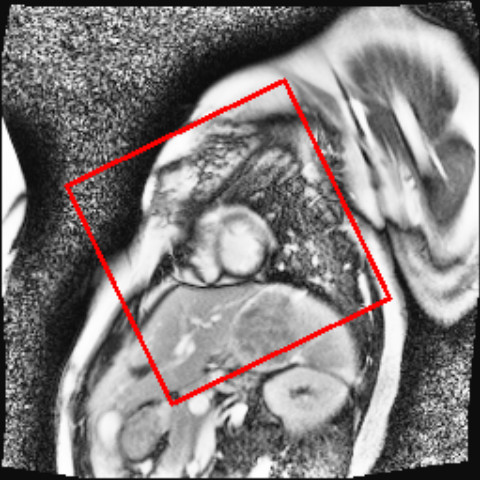
\includegraphics[width=0.19\textwidth]{./data/representative-results/control/HCMNet_2600035/00_SAX/APEX/0_bbox.png} &
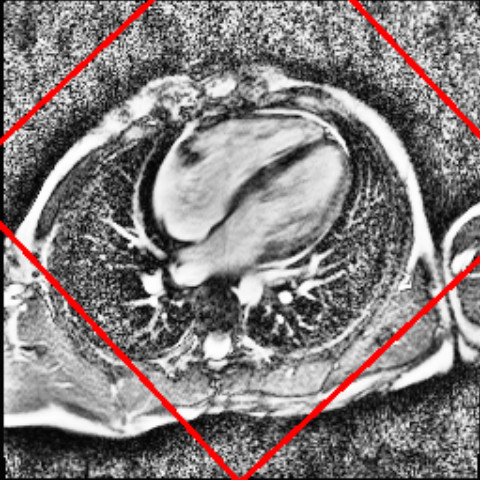
\includegraphics[width=0.19\textwidth]{./data/representative-results/control/HCMNet_1700012/01_HLA/00/0_bbox.png} &
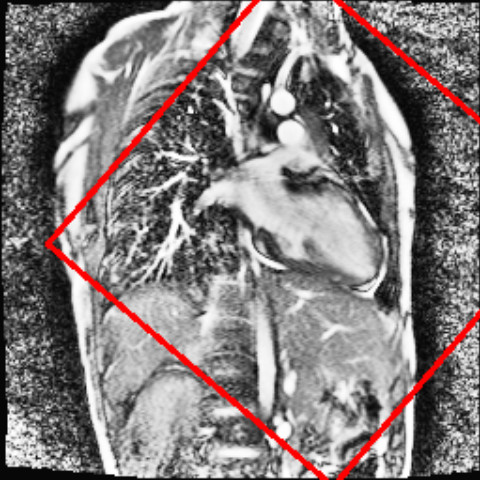
\includegraphics[width=0.19\textwidth]{./data/representative-results/control/HCMNet_1700012/02_VLA/00/0_bbox.png} \\

\multicolumn{5}{c}{在典型方向下的分割预测值:$S^\prime$} \\

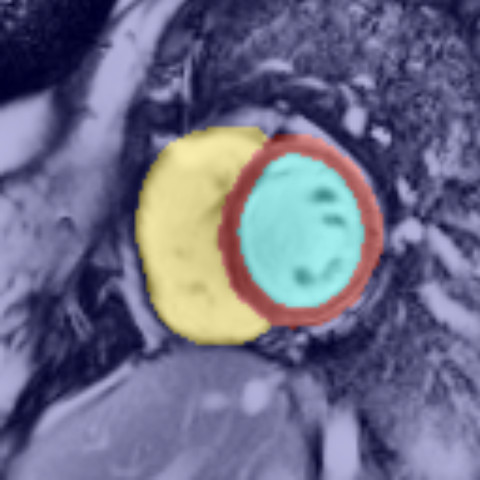
\includegraphics[width=0.19\textwidth]{./data/representative-results/control/HCMNet_2600035/00_SAX/BASE/0_pred.png} &
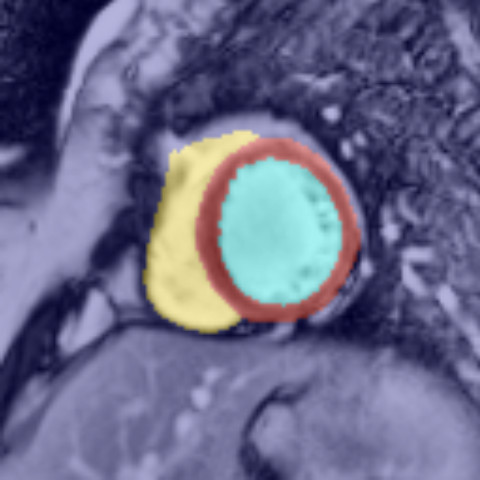
\includegraphics[width=0.19\textwidth]{./data/representative-results/control/HCMNet_2600035/00_SAX/MID/0_pred.png} &
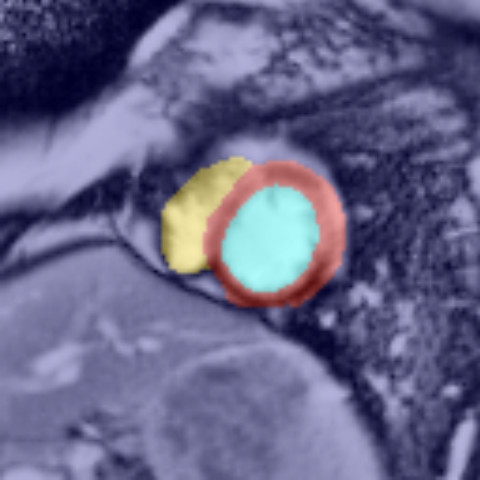
\includegraphics[width=0.19\textwidth]{./data/representative-results/control/HCMNet_2600035/00_SAX/APEX/0_pred.png} &
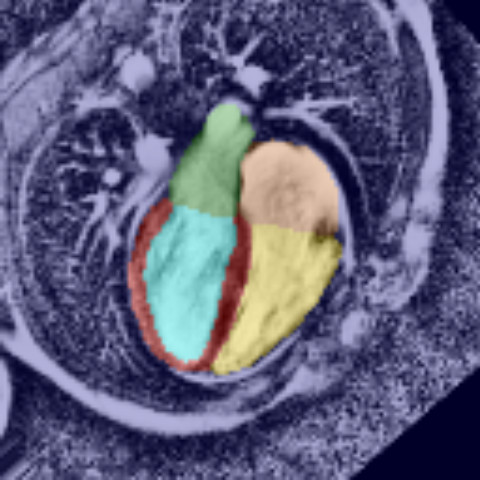
\includegraphics[width=0.19\textwidth]{./data/representative-results/control/HCMNet_1700012/01_HLA/00/0_pred.png} &
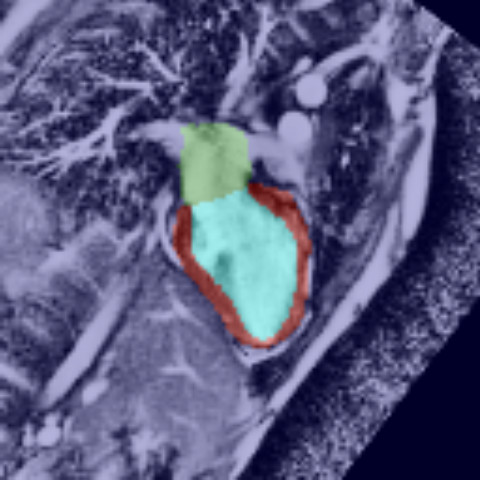
\includegraphics[width=0.19\textwidth]{./data/representative-results/control/HCMNet_1700012/02_VLA/00/0_pred.png} \\
\bottomrule

\multicolumn{5}{c}{在典型方向下的分割真实值:$\hat{S}^\prime$} \\

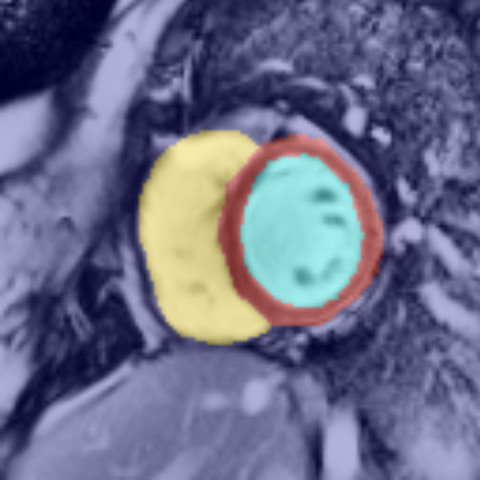
\includegraphics[width=0.19\textwidth]{./data/representative-results/control/HCMNet_2600035/00_SAX/BASE/0_gt.png} &
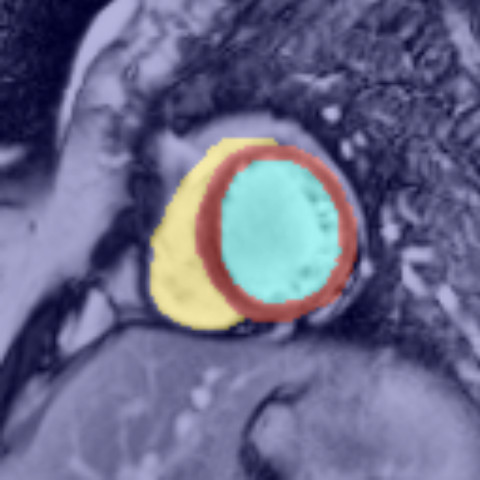
\includegraphics[width=0.19\textwidth]{./data/representative-results/control/HCMNet_2600035/00_SAX/MID/0_gt.png} &
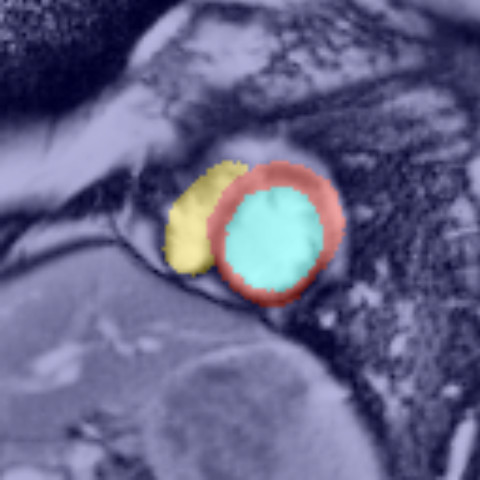
\includegraphics[width=0.19\textwidth]{./data/representative-results/control/HCMNet_2600035/00_SAX/APEX/0_gt.png} &
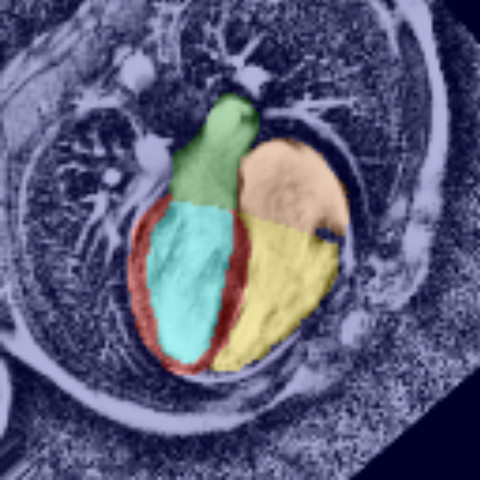
\includegraphics[width=0.19\textwidth]{./data/representative-results/control/HCMNet_1700012/01_HLA/00/0_gt.png} &
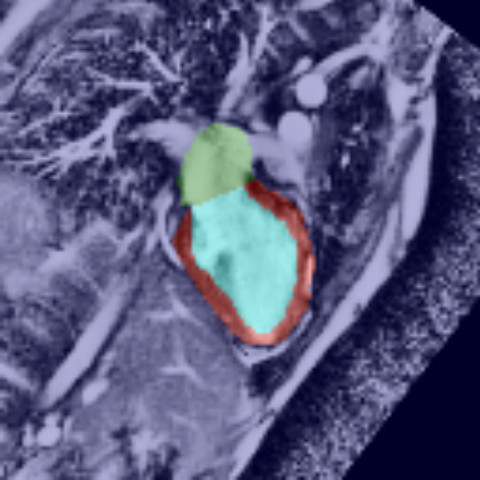
\includegraphics[width=0.19\textwidth]{./data/representative-results/control/HCMNet_1700012/02_VLA/00/0_gt.png} \\
\bottomrule

\end{tabular}

\caption[\captiontitle]{\captiontitle{}.详细讨论请参考正文内容.}
\label{fig:representative-results-control}
\end{center}
\end{figure*}
